\chapter{Methods}
\label{chapter:methods}

\section{Cross Industry Standard of Data Mining}
Data mining is a process of knowledge extraction or information discovery from a large number of data \citep{kurgan2006survey}. In this sense, one can argue that data mining is a blanket term for all kind of knowledge discovery processes including machine learning. For data mining to work, several technologies and techniques need to work together. Data mining incorporates various techniques and technologies like database management, computing infrastructure, statistical methods, data visualization, and communication. In order to successfully carry out knowledge discovery process one needs effective standards for various aspects of data mining.
 
Conceived by the consortium of multinational companies, Cross-Industry Standard of Data Mining (CRISP-DM) encapsulates a tried and tested method for data mining that builds upon previous attempts to define knowledge discovery methodologies. Although it is a somewhat old process conceived in 1996, the iterative process outlined in a CRISP-DM is still pragmatic in contemporary data science projects. Apart from being an iterative data-driven process, CRISP-DM also links the business understanding and objectives to data science projects. The inclusion of a business aspect to data mining adds a more nuanced business perspective to data science projects. CRISP-DM is one of the most popular and broadly adopted data mining models which has been acknowledged and relatively widely used in both research and industrial communities \citep{kurgan2006survey}. The figure~\ref{fig:Crisp process} below summarized the iterative process of CRISP-DM.

\begin{figure}[ht]
	\begin{center}
		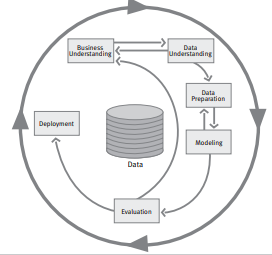
\includegraphics[width=7cm,height=7cm,keepaspectratio]{images/new_crisp.png}
		\caption{CRISP-DM process}
		\label{fig:Crisp process}
	\end{center}
\end{figure} 

CRISP-DM is a comprehensive process that starts with business understanding and ends with the final deployment of a data mining solution. Therefore it has various sub-steps within its main six phases. This thesis does not strictly follow the entire process because the primary objective of the thesis is not necessarily to obtain and deploy a production-level model but to find a way to improve the existing model with the help of data augmentation. Therefore, CRISP-DM is used as the reference model for developing and evaluating various machine learning algorithms built in the thesis.

\subsection{Business understanding}
All data science projects are a means to an end, the end usually being the business objective. To successfully carry out the data science project, a clear understanding of the underlying business objective is vital. So in this phase, the prime focus is on understanding the project objectives and requirements from a business perspective, then converting this knowledge into a data mining problem definition and data mining objective \citep{chapman2000crisp}. 

\subsection{Data understanding}
After understanding the business goal and setting the data mining objective next logical step is to collect and analyze the relevant data. This stage primarily deals with querying data from the database and checking whether the data is fit to carry out data mining process. Similarly, the first general insights are also discovered during this phase which helps to enhance the understanding of data at hand.

\subsection{Data preparation} 
Data in its raw-form cannot directly be used for modeling. Data needs to go through some preparatory steps.
Therefore this phase includes various activities undertaken to construct final data-set which will be fed into machine learning models. The first step often will be to clean the data, meaning remove the data that is corrupted, missing or unnecessary. Then if needed perform transformation such as normalization. This is also a phase where various augmentation techniques are applied to get the final data that is fed to the deep learning model.

\subsection{Modeling} 
This phase involves selecting the appropriate machine learning model which can achieve the goal outlined in the initial phase. Usually, various methods can be used to achieve the same goal. For example, one can use various machine learning strategies for classification task from simple logistic regression to convolutional neural network. Thus, different methods can be tested to determine the optimal method. This phase also includes designing testing set and some initial assessment of the model.

\subsection{Evaluation}
Once the modeling is completed models need to be evaluated. Before proceeding to deployment, the model needs to be thoroughly evaluated to make sure that it achieves the business objective and needs. Model evaluation can take several forms such as simple analysis of the accuracy of model's prediction on evaluation data, analyzing the complexities of the algorithm to the speed at which model takes time to execute. There is no one silver bullet for model evaluation as there are a variety of evaluation measures depending on the business objective and need. Thus, a model needs to evaluated based on the measure that most accurately reflects the business needs.

In this thesis, an entire chapter has been devoted to model evaluation as one of the crucial tasks of the thesis is to evaluate various machine learning models obtained through various augmentation techniques.   

\subsection{Deployment}
Once the suitable model meeting business needs is created, it needs to be deployed in the field. Depending on the objective of business it could be from as complicated as deploying machine learning model in a distributed cloud environment to as simple as generating a simple report for communicating and implementing the insights gathered from data mining process. Since model deployment is out of the scope of the thesis, it will not be discussed in subsequent chapters. 
 
 

